% This is samplepaper.tex, a sample chapter demonstrating the
% LLNCS macro package for Springer Computer Science proceedings;
% Version 2.20 of 2017/10/04
%
\documentclass[runningheads]{llncs}
%
\usepackage{graphicx}
\usepackage{amssymb}
\usepackage{amsmath}
\usepackage{multirow}
\usepackage{threeparttable}
% Used for displaying a sample figure. If possible, figure files should
% be included in EPS format.
%
% If you use the hyperref package, please uncomment the following line
% to display URLs in blue roman font according to Springer's eBook style:
% \renewcommand\UrlFont{\color{blue}\rmfamily}

\begin{document}
%
\title{Improving Counterfactual Regret Minimization Agents Training in card game Cheat Using Depth-limited Methods}
%
\titlerunning{Improving CFR Agents Training in Cheat Using Depth-limited Methods}
% If the paper title is too long for the running head, you can set
% an abbreviated paper title here
%
\author{Cheng Yi \inst{1} \and
Tomoyuki Kaneko\inst{1}}
%
\authorrunning{C. Yi et al.}
% First names are abbreviated in the running head.
% If there are more than two authors, 'et al.' is used.
%
\institute{Graduate School of Arts and Sciences, the University of Tokyo, Japan \email{yi-cheng199@g.ecc.u-tokyo.ac.jp}\\ \email{kaneko@acm.org}}
%
\maketitle              % typeset the header of the contribution
%
\begin{abstract}
Counterfactual Regret Minimization (CFR) has been one of the most famous iterative algorithms to solve imperfect information games but Vanilla CFR requires to traverse the whole game tree every iteration which is infeasible for most games in real life. In this paper we introduce an approach of creating smaller and simpler version of games by limiting the depth of the game tree and demonstrate how results from smaller games can improve training in larger ones. We conduct our experiments in an imperfect information card game called Cheat and limit the ``Health Points" a player has in each game to make the game easier to handle. We show this method helps us increase the learning rates of specific agents.

\keywords{Counterfactual Regret Minimization  \and Monte Carlo Sampling \and Imperfect Information Games.}
\end{abstract}
%
%
%
% Chapter 1
\section{Introduction}
% Imperfect information games

    In the Artificial Intelligence research area, we often see games as our challenge problems and solving them represents the research benchmarks and breakthroughs. There are two kinds of games, perfect information games and imperfect information games. In imperfect information games, such as bridge, Mahjong and most of poker games, players do not know everything about their opponents. The hidden aspect of the play is what makes imperfect information games a more challenging problem. One of the most important concepts in imperfect information games is called \textit{Nash Equilibrium} (NE). A NE is a strategy profile where no player can achieve a better result through converting their strategy unilaterally. The goal of most of researches is to reach the Nash equilibrium of the games. 
    
    \textit{Counterfactual Regret Minimization} (CFR) has lately become one of the most famous and widely-used iterative algorithms when dealing with imperfect information games. The main idea is to converge to a Nash Equilibrium based on the counterfactual regret calculation of every state on the game tree for the players. One of the shortage of this algorithm is that Vanilla CFR requires a traversal of the whole game tree on each iteration as it becomes infeasible when we are dealing with extremely large games. As a result, researchers have been looking for a better way to deal with infeasible large games in order to save computing cost. 

    In this paper we introduce a new approach of creating and adjusting the training environment of CFR agents to serve our purpose. We limit the total length of the game for simplification and aim at using results from simpler games in the larger games to speedup the iterations and achieve a better result. Besides, we also implement one of the MCCFR called Outcome-sampling MCCFR to help us improve the performance. In the next chapter we will talk about some background knowledge, then in Chapter 3 will cover some of the related previous works. Chapter 4 and 5 talk about our proposed methods, details of conduction and the results. In the last chapter, we summarize the whole paper and claim our expectation of the future direction of our research.

% Chapter 2
\section{Background}
\label{Bac}
    % 2.1
    \subsection{Notations and Terminology}
    % 2.1.1
    \subsubsection{Extensive Games~\cite{myerson2013game}}
    % Extensive form: players, history, action, payoff function
    A finite extensive game with imperfect-information is composed of the following elements:
    \begin{itemize}
        \item 
        A finite-size set of \textit{players}, $\mathcal{P}$. For player $i$, $-i$ represents all the players other than $i$. There is also a Chance player $c$, representing the actions which are not controlled by any player.
        \item 
        A \textit{history} $h \in \mathcal{H}$ is a node on the game tree, made up of all the information at that exact game state. A \textit{terminal history} $z\in\mathcal{Z}\subseteq\mathcal{H}$ is where there are no more available actions and each player will get a payoff value for what they have done following the game tree respectively.
        \item 
        We use $A$ to denote the \textit{action space} of the whole game and $A(h)$ is the set of all the \textit{legal actions} for players at the history $h$. If history $h'$ is reached after a player chooses action $a\in A(h)$ at history $h$, we can write $h \cdot a = h'$ or $h \sqsubseteq h'$.
        \item 
        An \textit{information set} (infoset) is a set of histories that for a particular player, they cannot distinguish which history they are in between one another. $\mathcal{I}_i$ represents the finite set of all the infosets for player $i$. Inherently, $\forall \, h, h'\in I, A(h)=A(h')=A(I)$. Note that any history $h \in \mathcal{H}$ must belong to exactly one of the information sets.
        \item 
        For each player $i\in\mathcal{P}$, there is a payoff function $u_i: \mathcal{Z} \rightarrow \mathcal{R}$ and especially in two-player zero-sum games, $u_1 = -u_2$. 
    \end{itemize}
    
    % Strategy
    In a game, a \textit{strategy} for player $i$ is $\sigma_i$ which assigns a distribution over their action space to each infoset of player $i$, particularly, $\sigma^t_i(I, a)$ for player $i$ maps the information set $I$ and the action $a\in A(I)$ to the probability that player $i$ will exactly choose action $a$ in the information set $I$ on iteration $t$. A strategy profile $\sigma = (\sigma_1,\dots,\sigma_n)$ is a tuple of all the players' strategies with one entry for each player where $\sigma_{-i}$ represents the strategies in $\sigma$ except $\sigma_i$. Let $\pi^\sigma(h)$ denote the \textit{reach probability} of reaching the game history $h$ while all the players follow the strategy profile $\sigma$. The contributions of player $i$ and all the players other than $i$ to this probability are denoted by $\pi^\sigma_i(h)$ and $\pi^\sigma_{-i}(h)$ respectively.
    
    % 2.1.3
    \subsubsection{Nash Equilibrium}
    \label{NE}

    Informally, we can say Nash Equilibrium is the ``best" strategy profile, since a player play following the NE can be seen as ``no lose". Here we will give the formal definition of NE. Let $(\Sigma,u)$ be a game with $n$ players, where $\Sigma = \Sigma_1 \times \Sigma_2 \times \dots \times \Sigma_n$ is the set of strategy profiles and $u(\sigma) = (u_1(\sigma), \dots, u_n(\sigma))$ is its payoff function defined over $\sigma \in \Sigma$. So Nash equilibrium can be now expressed as a strategy profile $\sigma^*$, in which every player is playing the best response. Formally, a strategy profile $\sigma^* \in \Sigma$ is a \textit{Nash Equilibrium} if,
    \begin{equation}
    \forall i, \sigma_i \in \Sigma_i : u_i(\sigma^*_i, \sigma^{*}_{-i}) \geq u_i(\sigma_i, \sigma^{*}_{-i})
    \end{equation}
    
    % 2.2
    \subsection{The Game \textit{Cheat}}
    \label{Cheat}
    
    \textit{Cheat} is a card game of lying and bluffing while also detecting opponents' deception. This game is often played among three or more players. At the beginning of the game, all the cards are well shuffled and dealt to the players as equally as possible. There are two phases in one turn of this game, \textit{Discard} phase and \textit{Challenge} phase. First of all, a random player is chosen to be the discard player and the ``current rank" which all the players share is set to be Ace.
    
    In the \textit{Discard} phase, the discard player discards card(s), puts them facing down on the table and makes a claim, including the number of cards they just discarded and the current rank. Players are supposed to discard cards only of the current rank but they can lie about their cards - either bluffing it out when they do not hold any correct cards, or choosing other cards even if they have the correct ones. Then in the \textit{Challenge} phase, if any other player thinks the discard player is lying, they can challenge them by saying ``Cheat!". When there is a challenge, the last discarded card(s) will be revealed to all players to see whether they are consistent with the claim. If the accused player did lie then they must take all the cards on the table back to their hands, otherwise the challenger takes the pile. If no one challenges, the card(s) remain(s) on the table. 
    
    For the next turn, we move to the next rank (K is followed by Ace) and next discard player. The one who first discards all the cards and survives the last challenge wins the game.

    % Chapter 2.2
    \subsection{Counterfactual Regret Minimization}
    
    Counterfactual Regret Minimization (CFR) was first propounded in 2008 by Zinkevich et al. in the paper~\cite{zinkevich2008regret} where the idea that claims minimizing overall regret can be used for approximating a Nash equilibrium in extensive games with incomplete information was demonstrated and proved. The basic steps of one iteration of vanilla CFR are the following: first, it keeps a record of the regret values for all actions (all zeros at the beginning) in each infoset; second, the values are used to generate strategies; third, the regret values are updated based on the new strategies. After all iterations, the average strategy obtained by normalizing overall actions belonging to the action space of this infoset, is proved to converge to the best strategy as time tends to infinity.
    
    Vanilla CFR requires traversals of the whole game tree in every iteration. The original Cheat (one deck of poker cards played between 2 players) has about $10^120$ decision points, so traversing the entire game tree even once is impossible and the computation is beyond the calculation power of ordinary computers. Another variant called Chance-sampled CFR (CS-CFR) is more common in practice, especially when dealing with poker or cards games. We see the results of dealing cards as Chance player's actions, and on each iteration, we only sample the action of Chance player.
    
    Marc Lanctot et al. introduces \textit{Monte Carlo CFR} (MCCFR), a domain-independent sample-based CFR algorithm in the study~\cite{lanctot2009monte}. They presented Outcome-Sampling and External-Sampling as two refined sampling schemes. It restricts the number of terminal histories we need to consider on every iteration. This approach helps us to avoid traversing the entire game tree but is still capable of keeping the expectation of counterfactual regrets unchanged. Hence, the improved algorithm can bring a faster convergence in various games.
    
% Chapter 3
\section{Related Previous Works}
    There have been many methods to help us tackle large games. For example, in the study~\cite{brown2018superhuman} and~\cite{brown2019superhuman}, researchers created Blueprint strategy for the agent Libratus and then improved it for its latest version called Pluribus. First an abstraction of the whole game is computed, then the solution to this abstraction is called Blueprint strategy. This strategy only has specific details for the early stage of the game and an approximation for later parts. The approximation will then self-improved as the game goes on and the agent get to know about opponent's actions.

    Most of the technique helps us save time and space of the whole game but remains unchanged at the early stage of the game. In 2015, Brown et al. first propounded an algorithm called \textit{simultaneous abstraction and equilibrium finding (SAEF)}~\cite{brown2015simultaneous} which does not rely on any domain knowledge but is only applicable in specific conditions. Then in 2016, a refined version of SAEF called \textit{Strategy-Based Warm Starting} was introduced in the study~\cite{brown2016strategy}. The new method expands the power of SAEF and is capable to skip the early expensive iterations of the game.

% Chapter 4
\section{Experiments}

    By analyzing the game rule, we can see that in order to win the game, we want to not only keep as fewer cards as we can in our hand, but also win more challenges. In other words, we want to challenge when we are more confident and discard cards in a more clever way. Based on this thought, we bring ``Health Point" (HP) into this game.
    
    In the original game, there is no restriction in how many times a player can lose challenges as long as no one discards all their cards. Now suppose each player has $n$ HP, which means they only has $n$ chances to lose the challenge. More specifically, when HP equals 1, it means if a player loses in the challenge once, the HP becomes 0 thus they loses the entire game (even if its opponent has not discarded all the cards).  We call Cheat with $n$ HP, Cheat-$n$. Through this, we introduce a sequence of smaller variants of Cheat, Cheat-$k$, where Cheat-$1$ is the smallest and Cheat-$\infty$ equals the original Cheat.
    
    By limiting HP, we created a technique of depth-limited training method. We propose to compute a smaller and easier version of the game, solve this game then map the strategies into a larger game, i.e. sequentially solve Cheat-$1$, Cheat-$2$, \dots, to get the strategy for the original Cheat. 

\subsection{Experimental Setups}
    \subsubsection{Mini-Cheat}
    The whole experiments were conducted in a simplified version of Cheat, naming \textit{Mini-Cheat}. In Mini-Cheat, we use cards of 3 ranks and 2 cards for each rank, i.e. 6 cards in total. There are 2 players in the game and we deal 2 cards to each player to eliminate the possibility of perfect information. In the following paragraph, ``Cheat-$n$" means Mini-Cheat with $n$ health points for each player, unless stated otherwise. Moreover, we found that the average number of challenges in one game without any restriction is about $3.5$, so we will start with Cheat-$3$, a simple but still strategically complex version of the game.
    
    \subsubsection{Testing bots}
    To value how our agents perform in different environments under various ways of training, we built two testing bots: Random bot and Heuristic bot. Random bot chooses all actions completely randomly. On the other hand, Heuristic bot was built based on human knowledge. It memorizes all the cards that were revealed in the game and keep a record of where they go if someone takes the pile on the table. As a result, it is quite strong and more accurate when challenging other players.
    
    \subsubsection{Agents}
    We tested four agents in our experiments: (1) Memoryless (M), which does not include either game history or HP information in its infosets; (2) HP-Aware (HPA), which is aware of Health Points but not game history; (3) History-Aware (HA), which is aware of game history but not Health Points; (4) General, which includes all the information that is available to a player can gain during the game. Similar with the naming of game environments, we call Memoryless agents which trained in Cheat-$n$, Memoryless-$n$. Same thing works for all the other agents.

\subsection{Results}
    We will compare all the agents in three aspects: first one is cost, including time consumption and storage space; second one is winning rates against two testing bots; third one is the effect of its results on other agents' training process.
    
    \subsubsection{Cost}
    Table\ref{tab:agents} shows the cost of four agents after 100 iterations of Chance-Sampled CFR. We can see that the time costs of four agents all increase exponentially as the game becomes more complex. The numbers of infosets of Memoryless agents stay constant. The growth of numbers of infosets of HP-Aware agent is exponential in powers of 2 while those of History-Aware and General agents are almost in power of 10. We also discover that the training of General agent becomes too complex for normal computer when the number of Health Points is 5 while in the original game this number is infinity.
    
    \begin{table}[htbp]
        \centering
        \setlength{\tabcolsep}{2.2mm}{
        \begin{threeparttable}
        \begin{tabular}{c|c|c|c|c|c|c|c|c}
        \hline
             & \multicolumn{2}{c|}{Memoryless} & \multicolumn{2}{c|}{HP-Aware} & \multicolumn{2}{c|}{History-Aware} & \multicolumn{2}{c}{General}\\
             \hline
              & Time\footnote{1} & Space\footnote{2} & Time & Space & Time & Space & Time & Space \\
              \hline
            Cheat-3 & 140 & 535 & 138 & 2013 & 524 & 13915 & 621 & 14027 \\
            \hline
            Cheat-4 & 2047 & 535 & 2166 & 4148 & 9092 & 144120 & 10297 & 161883 \\
            \hline 
            Cheat-5 & 33722 & 535 & 30184 & 7126 & 32145 & 1473428 & 38895 & 242801 \\
            \hline
            
        \end{tabular}
        
        \begin{tablenotes}
            \footnotesize
            \item[1] Time is in seconds.
            \item[2] Space is represented in the number of infosets.
            %\item[3] The experiment was almost infeasible.
        \end{tablenotes}
        
        \caption{Time and Space Costs of four agents}
        \label{tab:agents}
        \end{threeparttable}}
    \end{table}

    \subsubsection{Winning Rates}
    
    To value the learning efficiency and performance strength, we use the winning rate of Heuristic bot against Random bot as our baseline which is approximately 80\% (slightly varies in different game environments). The baseline will be represented in red line in the following graphs.
    
    We first test our agents against two testing bots every 5 iterations and then compare among different agents. Fig.\ref{fig:random} and \ref{fig:heuristic} reveal the trends of winning rates of four agents in Cheat-$3$ respectively. We notice that after 100 iterations, most agents become strong enough to exceed the baseline and especially, Memoryless-3 reaches almost 90\%. Meanwhile, Agents even beat Heuristic bot with winning rates over 60\% while Memoryless-3 reaches 75\%. We also notice that most agents have a much steep learning rate at the beginning of the training and is more steady in the later iterations. 
    
    Fig.3 and 4 demonstrate how agents perform in different game environments, while from HP-1 to HP-100, they play in the Mini-Cheat, and ``Large Game" means Cheat with cards of 7 ranks, 4 cards of each ranks and each player has 12 cards, i.e. a quite different and complex game. We can see that Memoryless player can perform well in the games that have larger number of HP while HP-Aware player only excel in the game environment that it was trained.
    
    \begin{figure}[htbp]
    \centering
    \begin{minipage}[t]{0.48\textwidth}
        \centering
        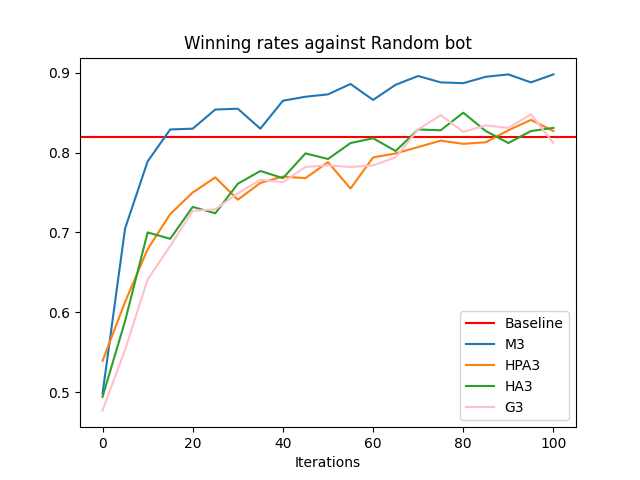
\includegraphics[width=\linewidth]{Winning_rates_against_random.png}
        \caption{Against Random bot}
        \label{fig:random}
    \end{minipage}
    \begin{minipage}[t]{0.48\textwidth}
        \centering
        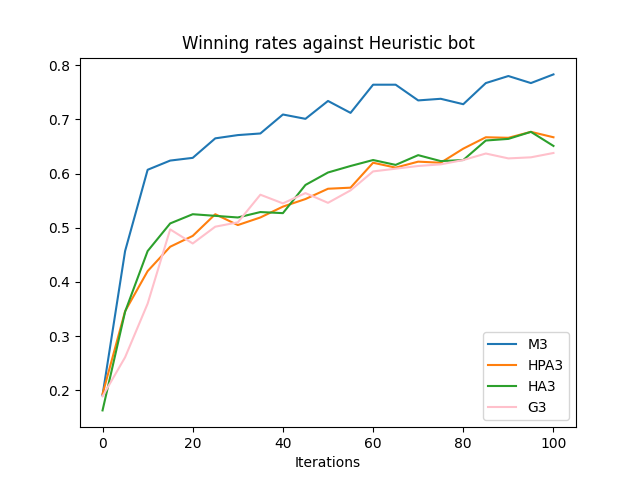
\includegraphics[width=\linewidth]{Winning_rates_against_heuristic.png}
        \caption{Against Random bot}
        \label{fig:heuristic}
    \end{minipage}
    \end{figure}
    
    \begin{figure}[htbp]
    \centering
    \begin{minipage}[t]{0.48\textwidth}
        \centering
        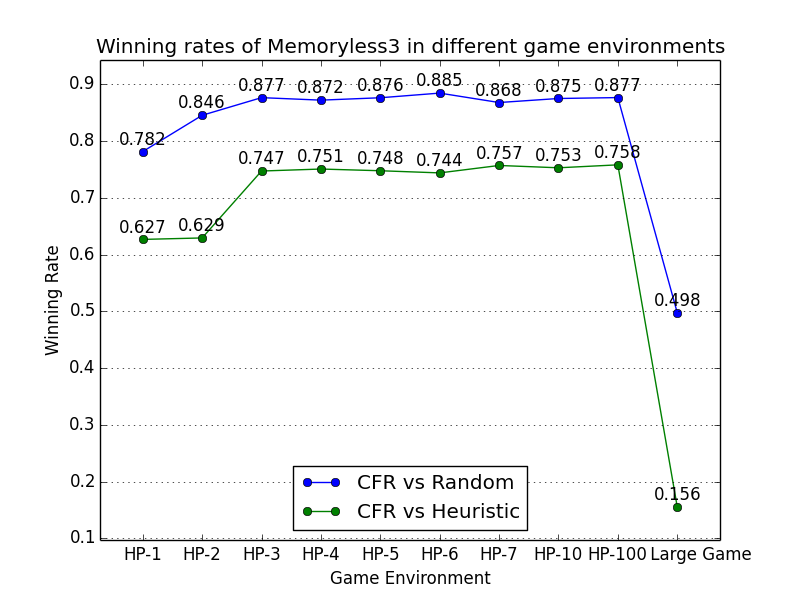
\includegraphics[width=\linewidth]{Memoryless_3_compare_bots.png}
        \caption{M3 in different games}
    \end{minipage}
    \begin{minipage}[t]{0.48\textwidth}
        \centering
        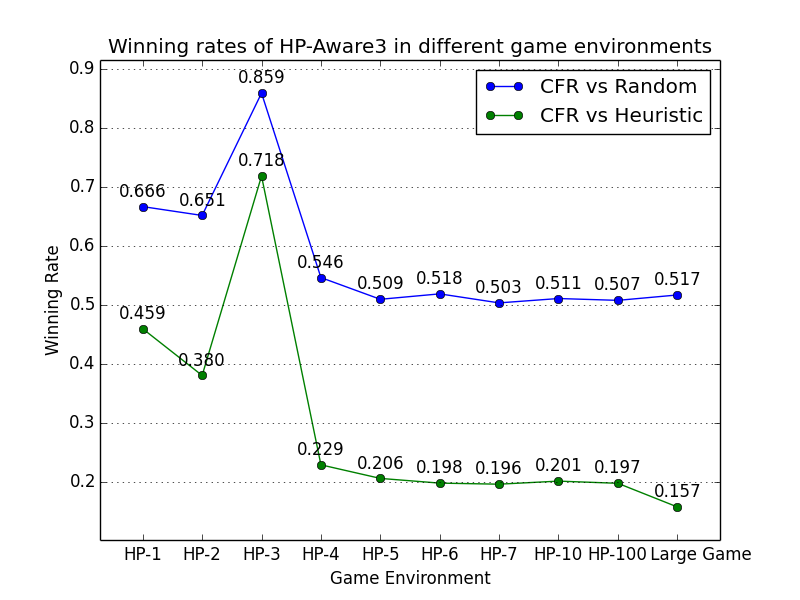
\includegraphics[width=\linewidth]{HPA_3_compare_bots.png}
        \caption{HPA3 in different games}
    \end{minipage}
    \end{figure}

    \subsubsection{Effect on further training}
    We then test the effect of agents trained in smaller games on those trained in larger games. Lighter lines represents agents trained from stretch while darker lines represents agents trained in Cheat-$n$ based on the infosets data from Cheat-$n-1$. For example, darker blue line in Fig.\ref{fig:M4} is the winning rate of Memoryless-4 using Memoryless-3's final strategy profile at the beginning of the training.
    
    From these graphs we can see that, the Depth-limited method works well for Memoryless and History-Aware agents, since the darker lines start at higher winning rates and always higher than the lighter ones. On the other hand, it is less useful for HP-Aware agents because the trends of lines of same type are almost same.

    \begin{figure}[htbp]
    \centering
        \begin{minipage}[t]{0.48\textwidth}
        \centering
    	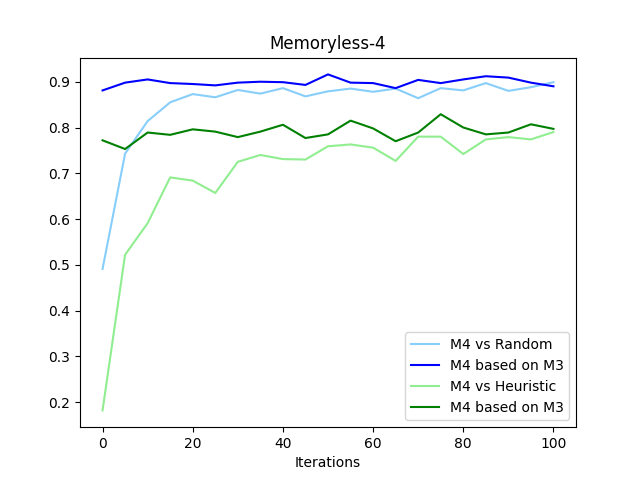
\includegraphics[width=\linewidth]{M4.png}
     	\caption{Memoryless-4}
     	\label{fig:M4}
    \end{minipage}
            \begin{minipage}[t]{0.48\textwidth}
        \centering
    	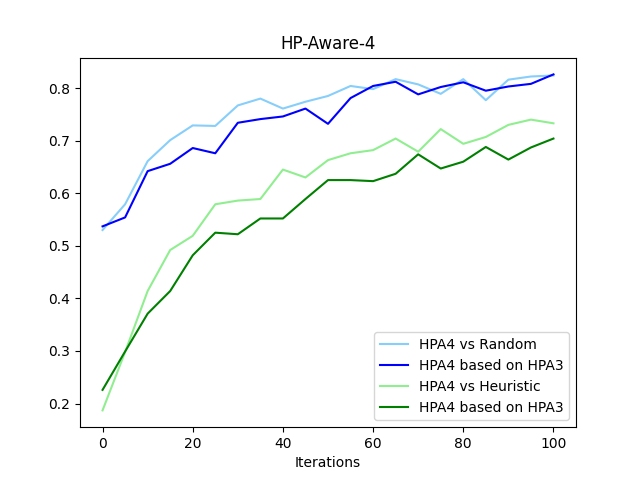
\includegraphics[width=\linewidth]{HPA4.png}
     	\caption{HP-Aware-4}
     	\label{fig:HPA4}
    \end{minipage}

    \end{figure}
    
        \begin{figure}[htbp]
    \centering
        \begin{minipage}[t]{0.48\textwidth}
        \centering
    	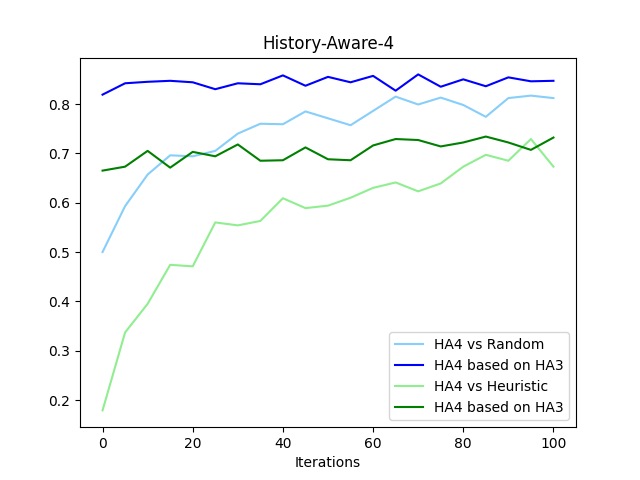
\includegraphics[width=\linewidth]{HA4.png}
     	\caption{History-Aware-4}
     	\label{fig:HA4}
    \end{minipage}
            \begin{minipage}[t]{0.48\textwidth}
        \centering
    	\includegraphics[width=\linewidth]{G4.png}
     	\caption{General-4}
     	\label{fig:G4}
    \end{minipage}

    \end{figure}

% Chapter 4
\section{Conclusion}
    Hereby, we introduce a method of creating simpler training environment by setting limitations on the depth of the game tree, especially in the game Cheat, an imperfect information card game, ``Health Point" which are used to limit the number of challenges a player can lose in one game. With help of this method, we first transfer larger Cheat games into smaller ones and hence training of chance-sampled CFR agents becomes feasible. Moreover, we also discover that we can utilize strategy profiles obtained in smaller games in the training of larger ones and as a result, the experiments show that there is an increase in the learning rates of specific agents.

    For the future, we also interested in including the Abstraction technique to further simplify the game thus it becomes feasible to tackle the original Cheat between two more even more players. Our final goal is to achieve the effect that we can utilize the result gained from $n-1$ situation in the training process for $n$ situation. The next step will be finding solid theoretical foundation to expand the range of this approach's practicality to other games. We are also interested in how our methods will work out in other games that have similar structure to create more reasonable training environments and speed up the training process. 

%
\bibliographystyle{splncs04}
\bibliography{mybibliography}

\end{document}
